%!TEX encoding = UTF-8 Unicode
\documentclass[ % options,
    a4paper,    % papersize
%    cjk,       % for cjk-ko
%    usedotemph,% for cjk-ko's \dotemph
    amsmath,    % load amsmath.sty to typeset math materials
    itemph,     % to disable gremph default (xe/lua)
%    footnote,  % korean style footnote
%    chapter,   % to use \chapter
]{oblivoir}     % xoblivoir and oblivoir are identical.

\ifPDFTeX       % latex, pdflatex
%    \usepackage{newtxtext}    % Latin fonts
\else\ifLuaOrXeTeX   % xelatex or lualatex
%  \setmainfont{TeX Gyre Termes}   %% Latin fonts
%	\setkomainfont(Noto Serif CJK KR)(* Bold)(* Medium)
%	\setkosansfont(Noto Sans CJK KR)(* Bold)(* Medium)
\fi\fi

% color 
\usepackage{xcolor}
\usepackage{titlesec}
\titleformat{\section}{\color{blue}\normalfont\Large\bfseries}{\color{blue}\thesection}{1em}{}
\titleformat{\subsection}{\color{orange}\normalfont\Large\bfseries}{\color{orange}\thesubsection}{1em}{}

% packages
\usepackage{kotex-logo}
\usepackage[utf]{kotex}
\usepackage{geometry}
 \geometry{
 a4paper,
 total={170mm,257mm},
 left=20mm,
 top=20mm,
 }
 
%% font packages and setup
\usepackage{fontspec}
\setmainfont{UnDotum}
\setsansfont{UnDotum}
\setmonofont{UnTaza}
\usepackage{dhucs-interword}
\interhword[.6]{.475}{.1}{.1}
\setlength{\parindent}{0em}
\setlength{\parskip}{1em}

% operator
\DeclareMathOperator*{\argmax}{argmax}
\DeclareMathOperator{\E}{\mathbb{E}}
\DeclareMathOperator*{\NAND}{\text{NAND}}

% image 
\usepackage{graphicx}

% page header
\usepackage{fancyhdr}
\pagestyle{fancy}
\rhead{신경망과 심층학습}

% box 
\usepackage{tcolorbox}

\begin{document}

\title{신경망과 심층학습}
\author{wisemountain}
\date{\today}

\maketitle

\newpage

\tableofcontents

\newpage

\section{What this book is about}

신경망은 매우 아름다운 프로그래밍 패러다임이다. 일반 프로그래밍과 다르게 
무엇을 할 지 하나씩 알려주는 것이 아니라 신경망은 데이터에서 학습하여 
해답을 찾아준다. 

이 책의 목적은 신경망의 핵심 개념들을 마스터할 수 있도록 도와주는 데 있다. 
이 책을 읽고 나면 신경망과 심층 학습을 사용하여 복잡한 패턴 인식 문제를 해결하는 
코드를 갖게 된다. 그리고 신경망과 심층 학습을 사용하여 자신만의 문제를 
해결할 수 있는 기반을 갖추게 된다. 

기반을 차근차근 연습을 포함하여 이해하도록 안내하는 224페이지 책이다. 
신경망 관련 책이자 웹 사이트인데 상당히 오래 되었고 꽤 오래 참조되고 있다. 

이 책의 내용을 소화하여 적는 방식으로 정리하려고 한다. 

\section{Using neural nets to recognize handwritten digits}

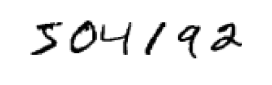
\includegraphics[scale=0.5]{image/1_hand_written_digits}

기계학습에서 전형적으로 시작하는 예제이다. 
사람에게는 매우 쉽다. 사람이 쉽게 인지 한다고 하지만 실제로는 V1이라 불리는 시각 영역에서 
1억4천만 개의 뉴런들이 수십억 개의 연결을 갖고 처리하고, 
이후의 더 많은 V2, V3, V4, V5 영역에서 각기 다른 정보를 추가로 처리한다. 

한편 이를 코딩으로 인식하는 프로그램을 작성한다고 해보면 매우 어렵다는 것을 알 수 있다. 
1 같은 매우 단순해 보이는 숫자도 손글씨에서는 매우 많은 변형이 있을 수 있고
노이즈도 추가될 수 있다. 7 같은 9와 3 같은 2를 어떻게 알고리즘으로 구분할 수 있을까? 

신경망에서는 전혀 다른 접근을 취하는데 훈련 집합이라고 부르는 미리 
답이 주어진 데이터로 훈련하고 실제 데이터를 판별하게 한다. 

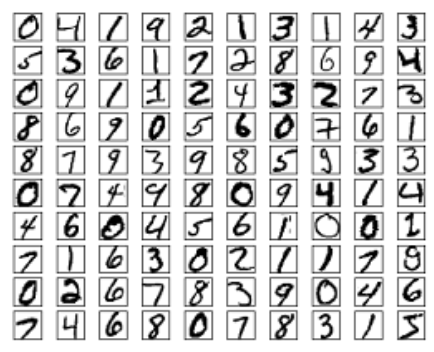
\includegraphics[scale=0.5]{image/2_training_set}

앞으로 손글씨로 쓴 숫자를 인식하는 프로그램을 작성하는데 74 줄의 프로그램이 
96\%의 확률로 사람의 도움 없이 동작하는 걸 확인하게 된다. 이후에 
이를 개선하여 99\%의 확률로 인식할 수 있게 만든다. 

\subsection{Perceptrons}

신경망이란 무엇인가? 먼저 인공 뉴런의 한 형태인 퍼셉트론을 소개한다. 
퍼셉트론은 Warren McColloch와 Walter Pitts에 이어 1950년 대에 
Frank Rosenblatt가 만들었다. 

현재는 시그모이드 뉴런이나 이와 비슷한 개량된 형태를 사용하는데 
먼저 퍼셉트론을 이해하여 기초로 삼는 동시에 왜 시그모이드 뉴런이 
필요한 지 함께 살펴본다. 

\begin{center}
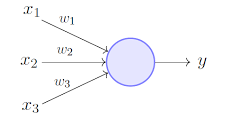
\includegraphics{image/3_perceptron}
\end{center}

책의 그림에는 가중치 $w_1, w_2, w_3$ 표시가 없어 다른 그림을 넣었다. 
퍼셉트론은 동그라미가 뉴런으로 하나의 뉴런만 있는 매우 단순한 구조이다. 

$y$가 퍼셉트론 뉴런의 출력값으로 입력값 $x_1, x_2, x_3$에 가중치를 곱하여 
더한 값을 특정 임계값 (threshold) 출력으로 삼는다. 


각 입력에 대한 가중치로 판단(분류)를 하는 간단한 뉴런으로 볼 수 있다. 

\begin{equation}
\text{output: y} = \begin{cases} 
				0 & \text{if } \sum_j x_j w_j \le threshold \\
				1 & \text{if } \sum_j x_j w_j > threshold 
				\end{cases}
\end{equation}


위와 같이 간단한 판단을 하는 퍼셉트론을 여러 개, 여러 층으로 구성하면 
더 복잡한 판단을 하는 기계를 구성할 수 있다. 이것이 심층 학습이 하는 
일이다. 

\begin{center}
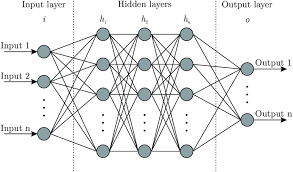
\includegraphics[scale=1.2]{image/4_deep_nn}
\end{center}

수식 (1)은 threshold를 일반적으로 부르는 bias로 변경하고
합을 내적으로 표현하여 다음과 같이 표현한다. 

\begin{equation}
\text{output: y} = \begin{cases} 
				& 0 \text{if } w \cdot x + b \le 0 \\
				& 1 \text{if } w \cdot x + b > 0  
				\end{cases}
\end{equation}

위와 같이 표현하면 가중치와 편향(bias) 값인 b로 선형 분류를 할 수 있다. 
$y = ax + b$와 같은 직선의 방정식 형태가 차원이 올라가면 평면, 초평면이 
되고 이 평면을 기준으로 위 아래로 나눌 수 있게 된다. 

이런 기능을 사용하여 간단한 NAND 회로를 구성할 수 있다. 

\begin{center}
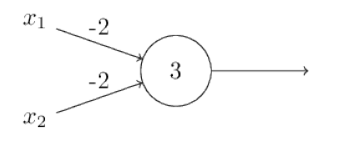
\includegraphics[scale=0.5]{image/5_nand}
\end{center}

그림은 $x1 \times -2 + x2 \times -2 + 3$ 을 사용하여 결과를 만드는 퍼셉트론(뉴런)이다. 

$x1$과 $x2$가 논리값을 갖고 0이 false, 1이 true로 표현된다고 하면, 
00에 대해서는 1, 01에 대해서 1, 10에 대해서 1, 11에 대해서 0이 되고
이는 $\neg (x1 \land x2)$에 해당하고 이런 함수가 NAND 이다. 

이런 퍼셉트론을 여러 개 연결하면 임의의 논리 함수를 만들 수 있다. 

\begin{center}
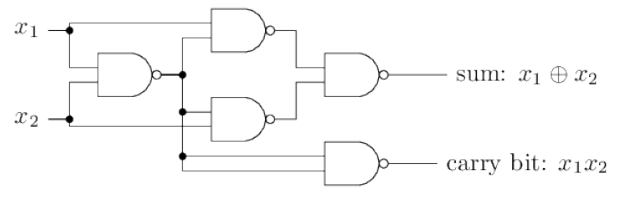
\includegraphics[scale=0.7]{image/6_bits_add}
\end{center}

위 NAND로 구성된 회로를 신경망 형태로 나타내면 아래와 같다. 

\begin{center}
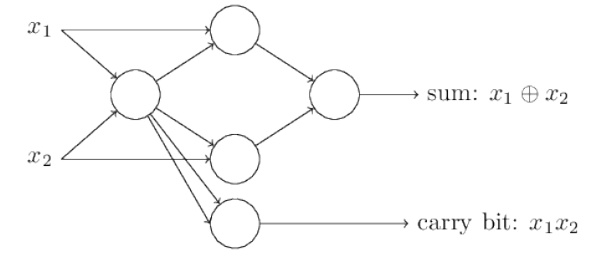
\includegraphics[scale=0.7]{image/6_bits_add_nn}
\end{center}

위에서 $x1 \bigoplus x2$는 비트 합이고, $x1 x2 = x1 \times x2$는 올림(carry bit)이다. 

NAND와 비트 연산으로 환원하여 결과가 제대로 나오는 지 하나씩 계산을 해보면
이해할 수 있고 좋은 연습문제이다. 

올림을 계산하는 $\NAND(\NAND(x1, x2), \NAND(x1, x2))$를 보면 $x1$과 $x2$가 모두 1일 경우만 
결과값이 1이 되는 걸 알 수 있고 이는 둘을 비트 곱을 한 것과 같다. 

sum에 해당하는 부분은 $\NAND(\NAND(x1, \NAND(x1, x2)), \NAND(x2, \NAND(x1, x2)))$이다. 
복잡해 보이지만 회로 설계의 영역이고 그 쪽에서는 또 다른 쉽게 만드는 방법들이 있을 것이다. 

\subsection{Sigmoid neurons}

\begin{center}
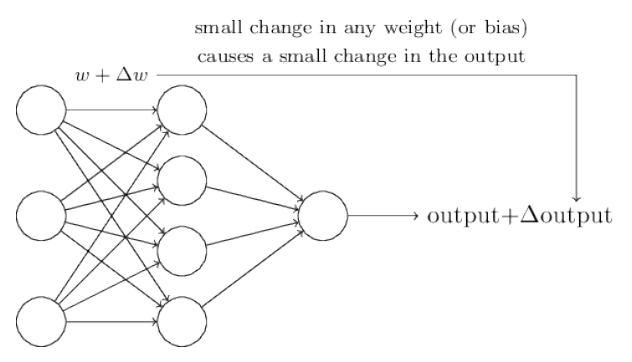
\includegraphics[scale=0.7]{image/7_continuity}
\end{center}



\end{document}
























